%% Begin slides template file
\documentclass[11pt,t,usepdftitle=false,aspectratio=169]{beamer}
\usepackage{graphicx}
\usepackage{amsmath}
\usepackage{algorithm}
\usepackage[noend]{algpseudocode}
\usepackage{hyperref}
\usepackage[export]{adjustbox}
\usepackage{listings}

\makeatletter
\def\BState{\State\hskip-\ALG@thistlm}
\makeatother

%% ------------------------------------------------------------------
%% - aspectratio=43: Set paper aspect ratio to 4:3.
%% - aspectratio=169: Set paper aspect ratio to 16:9.
%% ------------------------------------------------------------------

\usetheme[nototalframenumber,foot,logo]{uibk}
\setbeamertemplate{bibliography item}[text]

%% ------------------------------------------------------------------
%% - foot: Add a footer line for conference name and date.
%% - logo: Add the university logo in the footer (only if 'foot' set).
%% - bigfoot/sasquatch: Larger font size in footer.
%% - nototalslidenumber: Hide the total number of slides (only if 'foot' set)
%% - license: Add CC-BY license symbol to title slide (e.g., for conference uploads)
%% - licenseall: Add CC-BY license symbol to all subsequent slides slides
%% - url: use \url{} rather than \href{} on the title page
%% ------------------------------------------------------------------

%% ------------------------------------------------------------------
%% The official corporate colors of the university are predefined and
%% can be used for e.g., highlighting something. Simply use
%% \color{uibkorange} or \begin{color}{uibkorange} ... \end{color}
%% Defined colors are:
%% - uibkblue, uibkbluel, uibkorange, uibkorangel, uibkgray, uibkgraym, uibkgrayl
%% The frametitle color can be easily adjusted e.g., to black with
%% \setbeamercolor{titlelike}{fg=black}
%% ------------------------------------------------------------------

%\setbeamercolor{verbcolor}{fg=uibkorange}
%% ------------------------------------------------------------------
%% Setting a highlight color for verbatim output such as from
%% the commands \pkg, \email, \file, \dataset
%% ------------------------------------------------------------------


%% information for the title page ('short title' is the pdf-title that is shown in viewer's titlebar)
\title[Distributed Applications - Project Presentation]{Distributed Applications - Project Presentation}
\subtitle{Project 3 - Stock Price Prediction, 28.01.2020}
%%\URL{www.uibk.ac.at/statistics}

\author[Michael Kaltschmid \& Markus Reiter]{Michael Kaltschmid \& Markus Reiter}
%('short author' is the pdf-metadata Author)
%% If multiple authors are required and the font size is too large you
%% can overrule the font size of author and url by calling:
%\setbeamerfont{author}{size*={10pt}{10pt},series=\mdseries}
%\setbeamerfont{url}{size*={10pt}{10pt},series=\mdseries}
%\URL{}
%\subtitle{}

\footertext{Distributed Applications - Project Presentation - Team 10}
%\date{2019-05-07}

\headerimage{4}
%% ------------------------------------------------------------------
%% The theme offers four different header images based on the
%% corporate design of the university of innsbruck. Currently
%% 1, 2, 3 and 4 is allowed as input to \headerimage{...}. Default
%% or fallback is '1'.
%% ------------------------------------------------------------------

\begin{document}

%% ALTERNATIVE TITLEPAGE
%% The next block is how you add a titlepage with the 'nosectiontitlepage' option, which switches off
%% the default behavior of creating a titlepage every time a \section{} is defined.
%% Then you can use \section{} as it's originally intended, including a table of contents.
% \usebackgroundtemplate{\includegraphics[width=\paperwidth,height=\paperheight]{titlebackground.pdf}}
% \begin{frame}[plain]
%     \titlepage
% \end{frame}
% \addtocounter{framenumber}{-1}
% \usebackgroundtemplate{}}

%% Table of Contents, if wanted:
%% this requires the 'nosectiontitlepage' option and setting \section{}'s as you want them to appear here.
%% Subsections and subordinates are suppressed in the .sty at the moment, search
%% for \setbeamertemplate{subsection} and replace the empty {} with whatever you want.
%% Although it's probably too much for a presentation, maybe for a lecture.
% \begin{frame}
%     \vspace*{1cm plus 1fil}
%     \tableofcontents
%     \vspace*{0cm plus 1fil}
% \end{frame}


%% this sets the first PDF bookmark and triggers generation of the title page
\section{Bookmark Title}

\begin{frame}
\frametitle{Project Report}
    Team Members
    \begin{itemize}
        \item Michael Kaltschmid
        \item Markus Reiter
    \end{itemize}
\end{frame}

\begin{frame}
\frametitle{Introduction}
  \begin{itemize}
    \item Project 3 - Stock Price Prediction
    \item Programming Languages
      \begin{itemize}
        \item Rust
        \item TypeScript
      \end{itemize}
    \item Problem Motivation:
      \begin{itemize}
        \item Fetch stock prices, predict future prices and show a graph.
      \end{itemize}
  \end{itemize}
\end{frame}

\begin{frame}
  \frametitle{Wokflow Structure (AFCL)}
  \begin{center}
    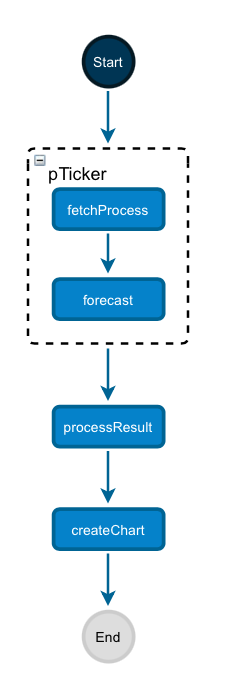
\includegraphics[height=6.7cm, keepaspectratio]{./assets/afcl}
  \end{center}
\end{frame}

\begin{frame}{Wokflow Structure (AFCL): Function Inputs/Outputs}
  \begin{itemize}
    \item \texttt{fetch\_prices}:   \\
      \textleftarrow\ \lstinline{\{"symbol": "IBM"\}}                                  \\
      \textrightarrow\ \lstinline{\{"symbol": "IBM", "object\_key": "IBM.json"\}}
    \item \texttt{forecast}:        \\
      \textleftarrow\ \lstinline{\{"symbol": "IBM", "object\_key": "IBM.json"\}}       \\
      \textrightarrow\ \lstinline{\{"symbol": "IBM", "object\_key": "IBM.forecast.json"\}}
  \end{itemize}
\end{frame}

\begin{frame}{Wokflow Structure (AFCL): Function Inputs/Outputs}
  \begin{itemize}
    \item \texttt{process\_result}: \\
      \textleftarrow\ \lstinline{\{"symbols": ["IBM"], "object\_keys": ["IBM.forecast.json"]\}} \\
      \textrightarrow\ \lstinline{\{} \\
        \lstinline{\ \ "labels": ["2021-01-01"], "datasets": [\{"label": "IBM", "data": [114.21]\}]} \\
        \lstinline{\}}
    \item \texttt{create\_graph}:   \\
      \textleftarrow\ \lstinline{\{} \\
        \lstinline{\ \ "labels": ["2021-01-01"], "datasets": [\{"label": "IBM", "data": [114.21]\}]} \\
        \lstinline{\}} \\
      \textrightarrow\ \lstinline{\{} \\
        \lstinline{\ \ "url": "https://quickchart.io/chart/render/zf-6eb3fb99-...-3566d22924cb"} \\
        \lstinline{\}}
  \end{itemize}
\end{frame}

\begin{frame}{Scheduler to CFCL}
  \begin{center}
    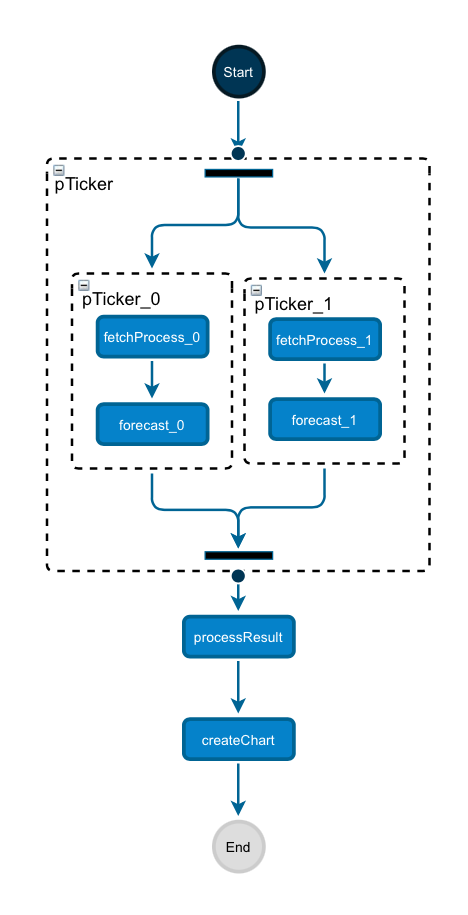
\includegraphics[height=6.7cm, keepaspectratio]{./assets/cfcl}
  \end{center}
\end{frame}

\begin{frame}{Scheduler to CFCL: Algorithm}
  \begin{itemize}
    \item Inputs: \texttt{iterations} and \texttt{concurrency\_limit}
    \item Variables: \texttt{concurrency\_limits} (\texttt{Map<String, usize>}), \\ \texttt{function\_iterations} (\texttt{Map<String, usize>}) and \\ \texttt{est} (\texttt{Map<String, (f64, f64)>})
    \item For \texttt{i} in \texttt{0...iterations}, loop through functions in \texttt{parallelFor} block:
      \begin{itemize}
        \item Look up FDs in database and insert function names in all maps if not already contained
        \item Sort FDs by the start time stored in \texttt{est} and loop through them:
          \begin{itemize}
            \item If FD has not yet reached the \texttt{concurrency\_limit} in \texttt{concurrency\_limits}, select it and update \texttt{concurrency\_limits}.
            \item Otherwise, reset the limit and increase the start time in \texttt{est}.
          \end{itemize}
    \end{itemize}
  \end{itemize}
\end{frame}

\begin{frame}
\frametitle{Helper tools}
    \begin{itemize}
        \item Build automation for Rust and JavaScript functions
          \begin{itemize}
            \item Run Cargo / Webpack
            \item Archive files
          \end{itemize}
        \item Deploy automation for testing purpouses
    \end{itemize}
    \vspace{1cm}
\end{frame}

\begin{frame}
\frametitle{Main Challenges}
    \begin{itemize}
        \item Forecast function
          \begin{itemize}
            \item Predictor creation
            \item Forecast creation
          \end{itemize}
        \item Periodic checking and waiting in the function itself
        \item Upload limitations with TerraForm
    \end{itemize}
\end{frame}

\begin{frame}
\frametitle{Demo}
    \begin{itemize}
        \item Present that your FC works
    \end{itemize}
\end{frame}

\begin{frame}
\frametitle{Testing Methodology}
    \begin{itemize}
        \item Experiment setup
        \item If you made some changes, justify them here
    \end{itemize}
\end{frame}

\begin{frame}
\frametitle{Evaluation}
    \begin{itemize}
        \item Present the speedup of distributed vs. sequential
        \item Explain whether the speedup / slowdown is expected / unexpected
    \end{itemize}
\end{frame}

\begin{frame}
\frametitle{Recommendation}
\end{frame}


%% to show a last slide similar to the title slide: information for the last page
%%\title{Thank you for your attention!}
%%\subtitle{}
%%\section{Thanks}


%% appendix of 'extra' slides
%%\appendix
\begingroup

{\footnotesize
\begin{frame}
  \frametitle{References}
  \begin{minipage}[t]{1\textwidth}
    % \begin{thebibliography}{9}
    %   \bibliofont
    %
    %   \bibitem{afcl}
    %     Ristov, S., Pedratscher, S. and Fahringer, T.
    %     \textbf{AFCL: An Abstract Function Choreography Language for serverless workflow specification.}
    %     \textit{Future Generation Computer Systems vol. 114, p. 368--382}, 2020.
    % \end{thebibliography}
    \vspace{1cm}
  \end{minipage}
\end{frame}
}

%% Additional slides
\begin{frame}
    \frametitle{Appendix}

\end{frame}
\endgroup

\end{document}
